\documentclass[a4paper]{article}
\usepackage[T1]{fontenc}
%\usepackage[swedish]{babel}
\usepackage[utf8]{inputenc}
\usepackage{lmodern}
\usepackage{fixltx2e}
\usepackage[fleqn]{amsmath}
\usepackage{amsmath}
\usepackage[pdftex]{graphicx}
\usepackage{listings}
\usepackage[]{mcode}
\usepackage[final]{pdfpages}
\usepackage{titling}

\newcommand{\subtitle}[1]{%
  \posttitle{%
    \par\end{center}
    \begin{center}\large#1\end{center}
    \vskip0.5em}%
}
\subtitle{Transmission properties in a short biased quantum wire}
\title{TFYA17 Project}

\author{Patrik Hallsj\"o, Felix Faber}
\date{}
\begin{document}

\maketitle

\section*{Abstract}
This project is dedicated to study an electron transport in a biased quantum wire. The potential used is similar to the potential in \cite{5}, but with an added bias voltage. The goals were to construct a solver for the potential and to calculate the transmission and reflection for an electron sent towards the potential. All the goals that were set up were solved.

\newpage
\section{Introduction}
The physics of low-dimensional semiconductor structures such as quantum wires and quantum point contacts has developed into an important part of nanotechnology, especially in connection with spintronics and quantum informatics.
Conductance in quantum wires quantum and quantum point contacts  made from split gate semiconductor heterostructures is quantized in steps of $2e^2/h$ \cite{1}.
This phenomenon may be explained in terms of non-interacting electrons and the stepwise occupation of higher sub-bands as the electron density is increased.
Each occupied sub-band contributes a fixed amount $2e^2 /h$  to the conductance where the factor of 2 comes from spin degeneracy.
Experiments have also revealed other conductance features, which may not be explained by a single-particle model.
The most well-know example is the 0.7 conductance anomaly  for which different explanations have been proposed \cite{2}.  In addition to 0.7 anomaly there are  0.25 and 0.85 non-linear conductance features that have been observed in the biased quantum wires \cite{3}.
In paper \cite{4} the model of spontaneous spin polarization was proposed to explain these anomalies.
This project deals with study of an electron transport in a short biased quantum wire. To model the quantum constriction in a quantum wire for this project it has been proposed to introduce a model potential that has been used in previous study \cite{5}.
By introducing a bias along the wire this potential can be modified to treat the electron transport in the case of biased wire.
The following goals have been specified to the project:
\begin{enumerate}
\item To set and to solve a problem with boundary conditions when an electron is injected into a wire.
\item To calculate the transmission and reflection coefficients as functions of energy of injected electron and bias.
\item To represent solutions in graphical form.
\item Optional: to calculate a conductance.
\end{enumerate}

\section{Experimental Details}
The experimental details only concern the coding in \textsc{Matlab}.
The calculation has been done in \textsc{Matlab} since it suited the purpose well and it is very straightforward and easy.
One drawback to using this is that the code can only be used on \textsc{Matlab} version 2013a or newer.
This is the main drawback of this work. One should note that the code can be written using for instance C++.
It is also important to note that speed of calculation was not prioritized and that the code is not well optimized.

\subsection{Theory}
%To be able to fulfill the goals the following theory was needed:
The potential that is used in this report is very similar to the potential used in \cite{5}, only that a bias has been added so the potential looks like \begin{equation}
\label{potential}
V(x) = \beta e V_{sd}+V_{g} tanh(s (x-dx_{1}))-(V_{sd}+V_{g}) tanh(s (x-dx_{2}))
\end{equation}
where $V_{sd}$ is the source-drain potential, $V_{g}$ the hight of the barrier and $\beta$ is a constant that will be set equal to $\frac{1}{2}$ for symmetric bias drop.
\subsubsection{Finite difference approximation}
A way to approximate a derivative is to use the so-called finite difference $f'(x) =\frac{f(x+h)-f(x+k)}{h-k}$, which is commonly used when the derivative of a function is calculated numerically. $h$ and $k$ are usually small and the limit $h,k->0$ is the derivative.
There are three variants of the finite difference that are the most commonly used i.e., forward derivation: $\frac{f(x+h)-f(x)}{h}$, backwards derivation: $\frac{f(x)-f(x-h)}{h}$ and central derivation $\frac{f(x+\frac{h}{2})-f(x-\frac{h}{2})}{h}$.

This type of approximation can be applied to higher order derivatives in the same way and if one applies the central derivation two times one will yield an approximation for the second order derivative $\frac{f(x-h)- 2f(x) +f(x+h)}{h^2}$.

\subsubsection{Finite steps in differential equations}

A second order differential equation without any first order terms can be written in the form $y''(x) = g(y(x),x)$ with boundary conditions $y(x_{0}) = y_{0}$ and $y(x_{N}) = y_{N}$, on the interval $[x_{0},x_{N}]$. The derivative $y''(x)$ can be replaced the with the central finite difference approximation with $h = d$ and $x = n*d$, to yield $d*g(y(n*d),n*d) + 2y(n*d)-(y((n+1)*d)+y((n-1)*d)) = 0$. This is a system of $N+1$ equations with $N+1$ unknowns so it will have one unique solution which can be found by using linear algebra.

\subsubsection{Quantum barrier problem}

In the problem at hand, we want to find the transmission and reflection of an electron current through the potential \eqref{potential}. This means that we need to solve the stationary Schr\"odinger equation with the boundary conditions $y_{0} = (I + R)\exp{(-i k x_{0})}$ and $y_{N} = T\exp{(-i k x_{N})}$ where $|T|^2,|R|^2$ and $|I|^2$ are the probabilities for the transmitted, reflected and incoming particle. We have put $I=1$, which gives $y_{0} = (1 + R)\exp{(-i k x_{0})}$ to make the equations easier to solve.

We can use the finite difference approximation to solve the stationary Schr\"odinger equation as a second order ordinary differential equation (ODE). However, with $R$ and $T$ we have $N+3$ unknowns but only $N+1$ equations. Two more equations will be needed in order to fully solve the problem.

The solution to Schr\"odinger equation is continuous everywhere in the interval because it is a second order ODE, however it also needs to be continuous at the two boundaries. The finite difference approximation of the derivative yields: $y'_{0}=y'_{1}$ and $y'_{N-1}=y'_{N}$. There are now $N+3$ unknowns and $N+3$ equations which will have a unique solution.


\subsection{Code}
We have developed the code based on the theory outlined above which calculates the conductance for a certain potential. It also plots both the potential and the wave-function that are calculated by solving the Schr\"odinger equation.
The code can be used for calculating any potential. However, in this project a specific potential, \eqref{potential}, was of interest.


In the code, by default, $V_{sd}$ and $V_g$ are specified as $0.3$, $x_2$ and $x_1$ are equal to 6 and 4 respectively.
For the user, the energy of the incoming electron E, the size of steps to divide the interval in, the value of s in \eqref{potential} for the potential and also the colour of the plot should be specified. Details can be found in the code description in the appendix.

\section{Results}
Running the code for certain values of E, $\beta$, $x_1$, $x_2$, $V_{sd}$, $V_g$ results in the following images of the wave-functions and the potential barriers, where the code has been run three times with different s parameters for each plot.
\begin{figure}[h!]
\centering
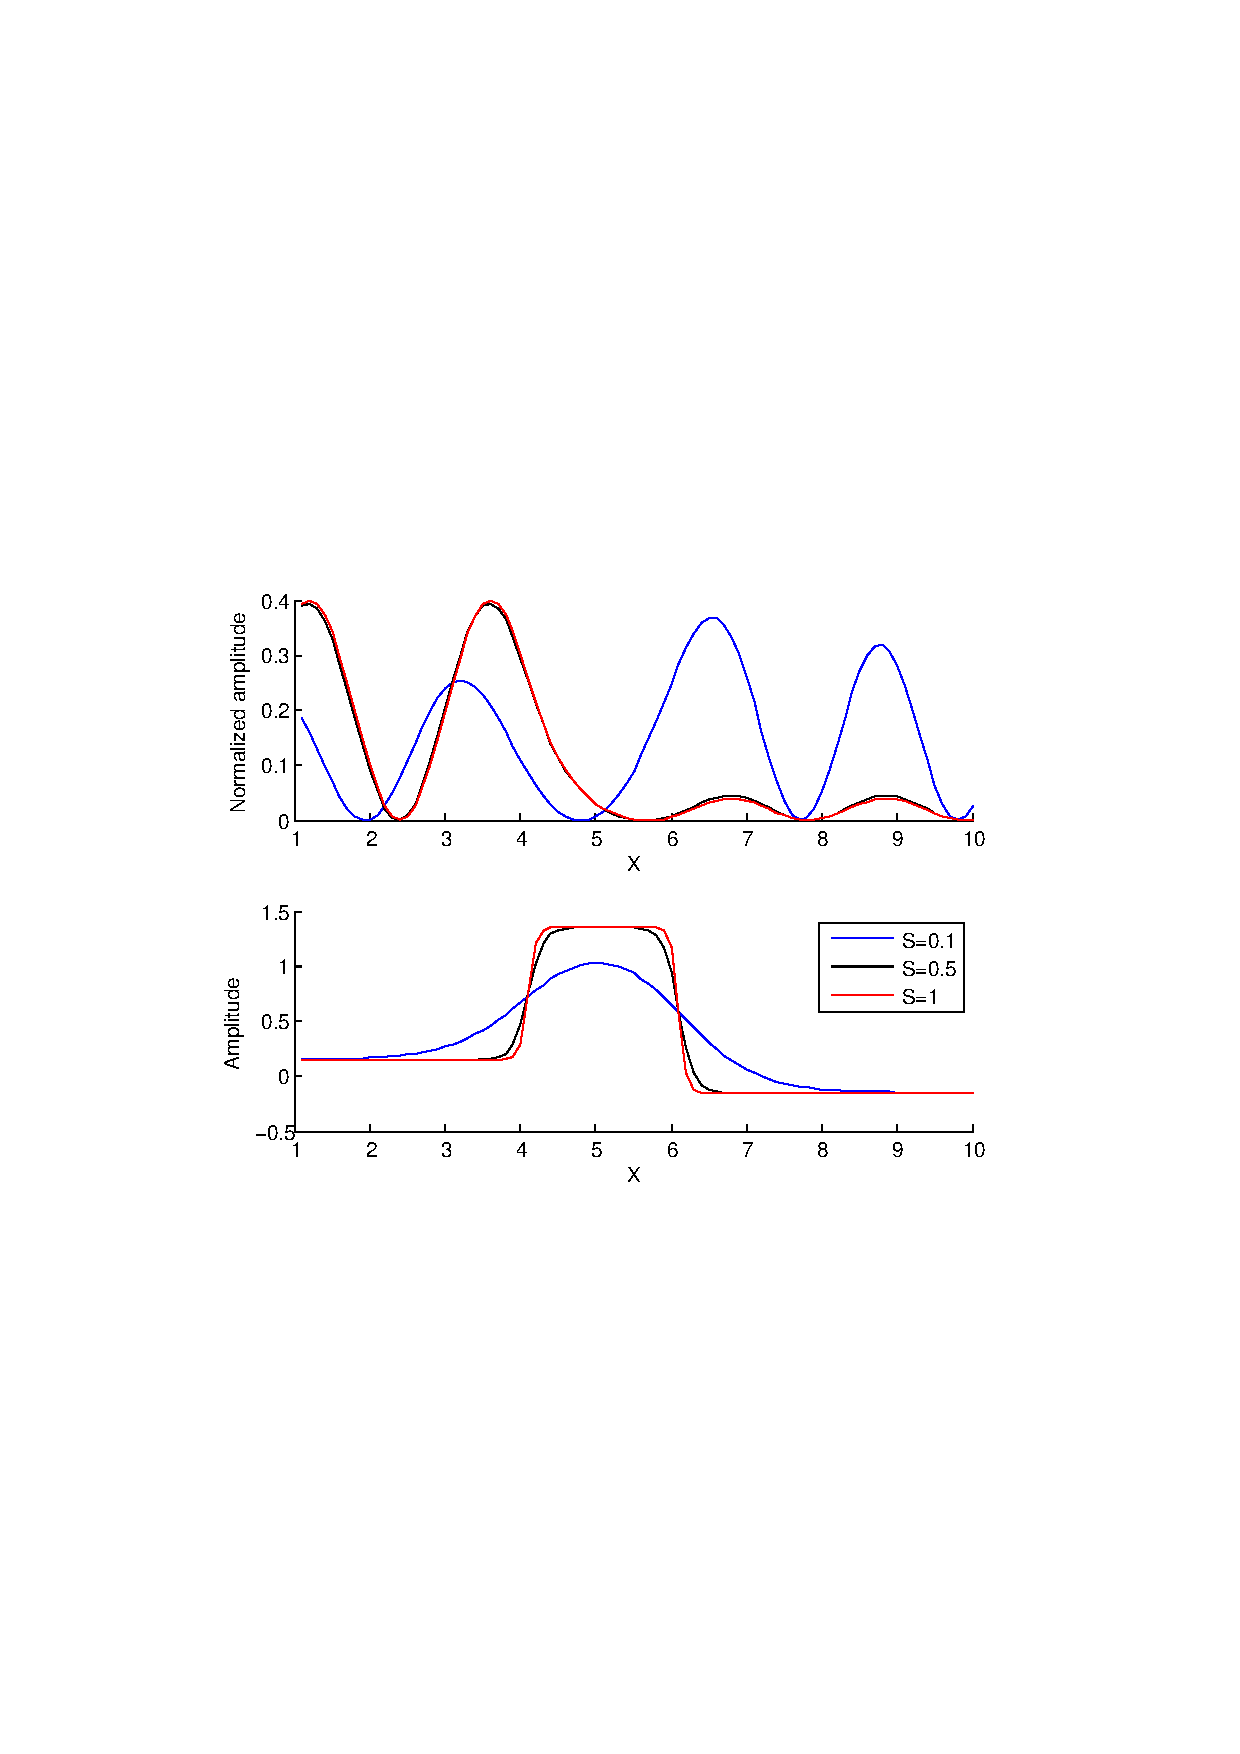
\includegraphics[width=4.3in]{test}
\caption{Amplitudes of wave-functions (upper graph) and potential barriers (lower graph) for the case: E=1, $\beta=0.5$, $x_1=4$, $x_2=6$, $V_{sd}=0.3$, $V_g=0.6$}
\label{fig:test}
\end{figure}
\newpage
\begin{figure}[h!]
\centering
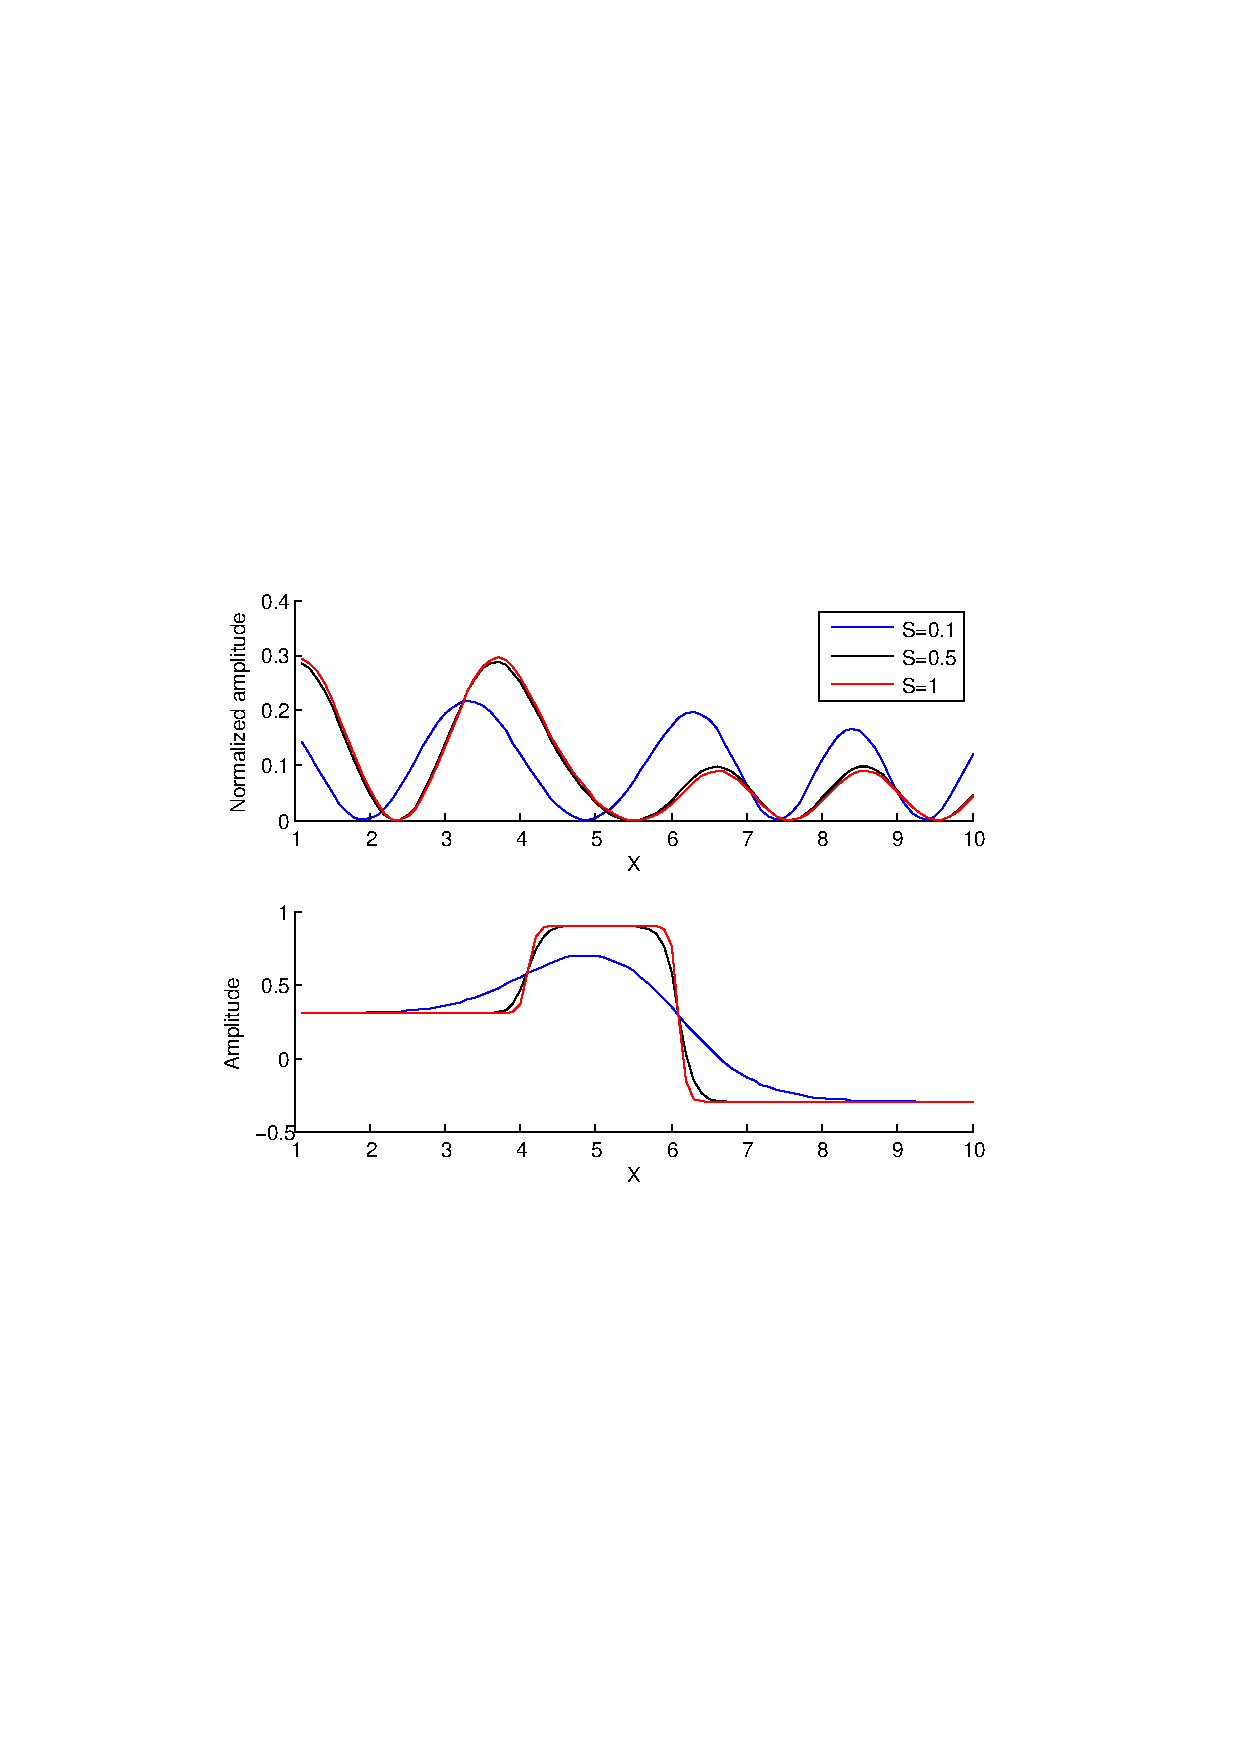
\includegraphics[width=4.5in]{test2}
\caption{Amplitudes of wave-functions (upper graph) and potential barriers (lower graph) for the case: E=1, $\beta=0.5$, $x_1=4$, $x_2=6$, $V_{sd}=0.6$, $V_g=0.3$}
\label{fig:test2}
\end{figure}
\newpage
\begin{figure}[h!]
\centering
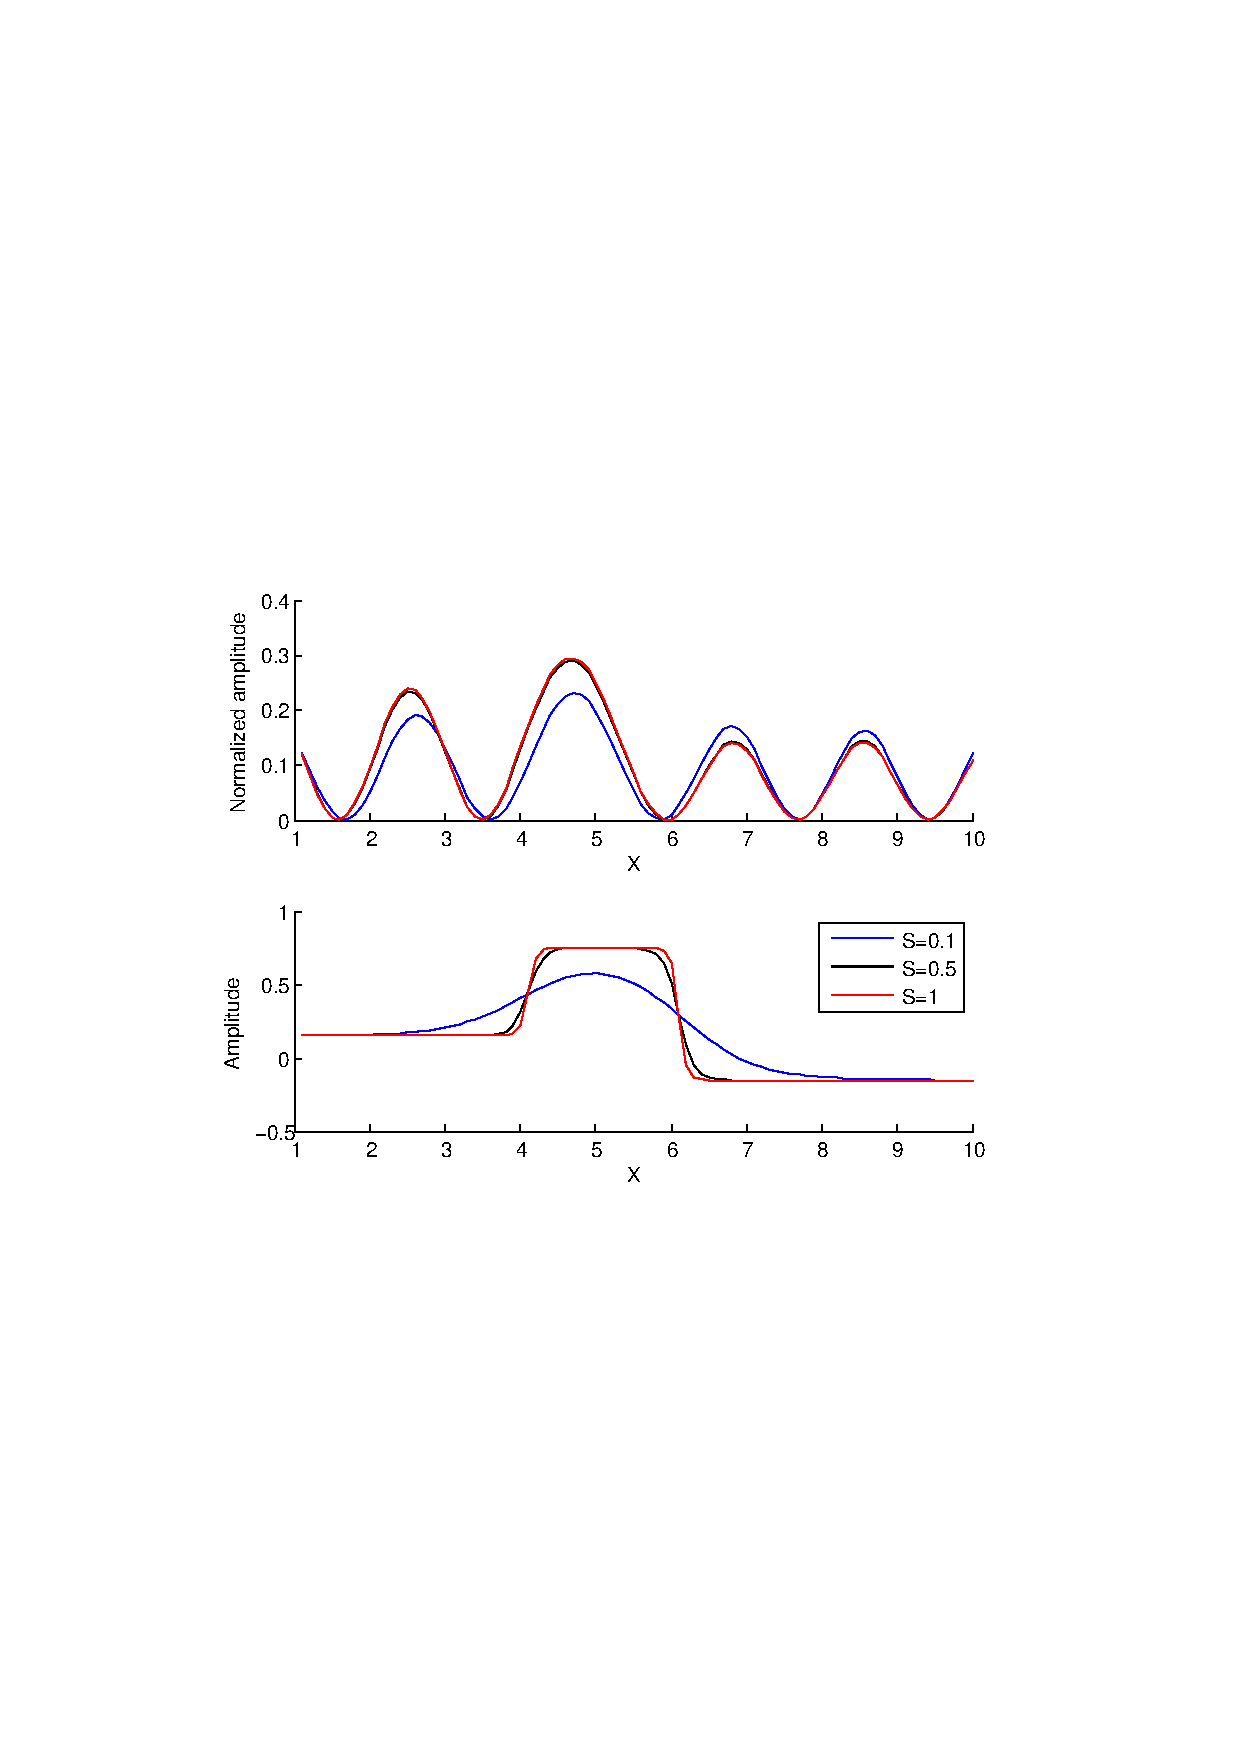
\includegraphics[width=4.5in]{test3}
\caption{Amplitudes of wave-functions (upper graph) and potential barriers (lower graph) for the case: E=1.5, $\beta=0.5$, $x_1=4$, $x_2=6$, $V_{sd}=V_g=0.3$}
\label{fig:test3}
\end{figure}

The code also calculates the conductance for each run, by calculating the reflection and transmission coefficients and using the following relation:
\begin{eqnarray*}
R=|R|^2/(|R|^2+|T|^2)\\
T=|T|^2/(|R|^2+|T|^2)\\
C = T/(R+T)
\end{eqnarray*}

\section{Discussion}


The code can most likely be optimized to run faster if one has enough time, however we prioritized getting a working code. The main reason for the long computing time is that several different \textsc{Matlab} packages were used. In a longer project a good idea would be to create a code using in C++ or any other usual programming language.


Computing power was a problem in the beginning. The reason where that we only had access to sun-ray computers with minimal computing power in the school, however we got access to research computers with a lot more computing power at the end of the course. The research computers were very helpful to produce a lot of graphs and they also had newer versions of \textsc{Matlab} that ran better with the code. One thing that needs to be improved is the routines that are in place for students to gain access to the research computers.


For the potential given in this report there were no references of what results that were expected. However for known solutions, (radial potential, harmonic oscillator, etc.) the code has been tested and the results given were exactly as predicted.

\subsection{Analysis of the figures}
The figures show the potentials and wave-functions for different input parameters. As discussed above, calculations give the expected results for well-known potentials.

The solutions are similar to those of an electron sent through a square potential,
especially in the limit $ s \rightarrow \infty $ as can be seen in figure 1. The conductance increases as $V_g$ becomes smaller. Resonances can occur for certain parameters inside potential (no pictures are shown of this though), especially when s is large. The probability for seeing the particle is greatly increased in these resonances.
 

\section{Conclusion}

The goals are listed below and it is commented the results achieved:
\begin{itemize}
\item To set and to solve a problem with boundary conditions when an electron is injected into a wire.
\end{itemize}
Done through the code by solving the Schr\"odinger equation and with that solution imposing boundary conditions.
\begin{itemize}
\item To calculate the transmission and reflection coefficients as  functions of energy of injected electron and bias.
\end{itemize}

The code was able to calculate the transmission and reflection from the solution. There are however, no specific examples of the calculated transmission or reflection shown in this article.


%This is done in the same way as above, however not explicitly provided. At present only the conductance is calculated through this, though the code provides writing out transmission and reflection coefficients.
\begin{itemize}
\item To represent solutions in graphical form.
\end{itemize}
Done through the graphs plotted under Results.
\begin{itemize}
\item Optional: to calculate a conductance.
\end{itemize}
This was also discussed under Results.
\\\\
In conclusion,  we have achieved all the goals that were set up for the project, even the optional part.  The code could have been optimized to improve speed, but we judged that the speed is sufficient.

\newpage
\bibliographystyle{unsrt}
%\nocite{1}
%\nocite{2}
%\nocite{3}
%\nocite{4}
%\nocite{5}

\bibliography{ourrefs}
\newpage
\part*{Appendix}
%Appendix with matlab code! - Patrik

\lstinputlisting[language=Matlab]{Schrodinger.m}

\end{document}
